\documentclass[notes,10pt, aspectratio=169]{beamer}

\usepackage{pgfpages}
% These slides also contain speaker notes. You can print just the slides,
% just the notes, or both, depending on the setting below. Comment out the want
% you want.
\setbeameroption{hide notes} % Only slide
%\setbeameroption{show only notes} % Only notes
%\setbeameroption{show notes on second screen=right} % Both
\usepackage{colortbl}
\usepackage{helvet}
\usepackage[default]{lato}
\usepackage{array}
\usepackage{eurosym}
\usepackage{setspace}
\usepackage{animate}
\usepackage{multicol}
\usepackage{breqn}
\usepackage{subcaption}
\usepackage{caption}
\captionsetup{font=scriptsize, justification=raggedright,singlelinecheck=false}
\usepackage[export]{adjustbox}
\usepackage[scale=2]{ccicons}
\usepackage{tikz}
\newenvironment{wideitemize}{\itemize\addtolength{\itemsep}{10pt}}{\enditemize}
\usepackage{natbib}

\usepackage{tikz}
\usepackage{verbatim}
\setbeamertemplate{note page}{\pagecolor{yellow!5}\insertnote}
\usepackage{amsmath}
%\usepackage{mathpazo}
\usepackage{hyperref}
\usepackage{lipsum}
\usepackage{multimedia}
\usepackage{multirow}
\usepackage{graphicx}
\usepackage{dcolumn}
\usepackage{bbm}
\newcolumntype{d}[0]{D{.}{.}{5}}

\usepackage{changepage}
\usepackage{appendixnumberbeamer}
% \newcommand{\beginbackup}{
%   \newcounter{framenumbervorappendix}
%   \setcounter{framenumbervorappendix}{\value{framenumber}}
%   \setbeamertemplate{footline}
%   {
%      \leavevmode%
%      \hline
%      box{%
%       \begin{beamercolorbox}[wd=\paperwidth,ht=2.25ex,dp=1ex,right]{footlinecolor}%
% %         \insertframenumber  \hspace*{2ex} 
%       \end{beamercolorbox}}%
%      \vskip0pt%
%   }
%  }

 \setbeamertemplate{footline}{
    \hbox{%
    \begin{beamercolorbox}[wd=\paperwidth,ht=3ex,dp=1.5ex,leftskip=2ex,rightskip=2ex]{page footer}%
        %\usebeamerfont{title in head/foot}%
        %\insertshorttitle \hfill
        %\insertsection \hfill
        %\tableofcontents[currentsection] \hfill
        \insertsectionnavigationhorizontal{0.7\paperwidth}{}{} \hfill 
        \insertframenumber{} / \inserttotalframenumber
    \end{beamercolorbox}}%
}
\newcommand{\backupend}{
   \addtocounter{framenumbervorappendix}{-\value{framenumber}}
   \addtocounter{framenumber}{\value{framenumbervorappendix}} 
}

\useinnertheme[shadow]{rounded}
\setbeamercolor{block title example}{fg=black,bg=orange!50!white}
\setbeamercolor{block body example}{fg=black, bg=orange!30!white}
\setbeamercolor{block title}{use=structure,fg=structure.fg,bg=structure.fg!20!bg}
\setbeamercolor{block body}{parent=normal text,use=block title,bg=block title.bg!50!bg}

\newcommand\independent{\protect\mathpalette{\protect\independenT}{\perp}}
\def\independenT#1#2{\mathrel{\rlap{$#1#2$}\mkern2mu{#1#2}}}

\usepackage{graphicx}
\usepackage[space]{grffile}
\usepackage{booktabs}

% These are my colors -- there are many like them, but these ones are mine.
\definecolor{blue}{RGB}{0,114,178}
\definecolor{red}{RGB}{213,94,0}
\definecolor{yellow}{RGB}{240,228,66}
\definecolor{green}{RGB}{0,158,115}

\setbeamercolor{section in head/foot}{fg=blue}


\hypersetup{
  colorlinks=false,
  linkbordercolor = {white},
  linkcolor = {blue}
}


%% I use a beige off white for my background
\definecolor{MyBackground}{RGB}{255,253,218}

%% Uncomment this if you want to change the background color to something else
%\setbeamercolor{background canvas}{bg=MyBackground}

%% Change the bg color to adjust your transition slide background color!
\newenvironment{transitionframe}{
  \setbeamercolor{background canvas}{bg=yellow}
  \begin{frame}}{
    \end{frame}
}

\setbeamercolor{frametitle}{fg=blue}
\setbeamercolor{title}{fg=black}
%\setbeamertemplate{footline}[frame number]
\setbeamertemplate{navigation symbols}{} 
\setbeamertemplate{itemize items}{-}
\setbeamercolor{itemize item}{fg=blue}
\setbeamercolor{itemize subitem}{fg=blue}
\setbeamercolor{enumerate item}{fg=blue}
\setbeamercolor{enumerate subitem}{fg=blue}
\setbeamercolor{button}{bg=white,fg=blue,}



% If you like road maps, rather than having clutter at the top, have a roadmap show up at the end of each section 
% (and after your introduction)
% Uncomment this is if you want the roadmap!
% \AtBeginSection[]
% {
%    \begin{frame}
%        \frametitle{Roadmap of Talk}
%        \tableofcontents[currentsection]
%    \end{frame}
% }
\setbeamercolor{section in toc}{fg=blue}
\setbeamercolor{subsection in toc}{fg=red}
%\setbeamersize{text margin left=1em,text margin right=1em} 
\setbeamersize{text margin left=0.7cm,text margin right=0.7cm} 


\title[]{\textcolor{blue}{Lecture 6:\\Inference and Interpretation}}
\author{25117 - Econometrics}
\institute[shortinst]{Universitat Pompeu Fabra}

\date{October 23rd, 2024}

\begin{document}

\begin{frame}[plain]
\maketitle
\end{frame}


\begin{frame}{What we learned in the last lesson}
\begin{itemize}
    \item Omitted variable bias occurs when an omitted variable (a) is correlated with an included regressor and (b) is a determinant of $Y$.\\[1em]
    \item The multiple regression model is a linear regression model that includes multiple regressors, $X_1, \dots, X_k$. Associated with each regressor is a regression coefficient, $\beta_1, \dots, \beta_k$.\\[1em]
    \item The coefficient $\beta_1$ is the expected difference in Y associated with a one-unit difference in $X_1$, holding the other regressors constant. The other regression coefficients have an analogous interpretation.\\[1em]
\end{itemize}
\end{frame}

\begin{frame}{What we learned in the last lesson}
\begin{itemize}
    \item The coefficients in multiple regression can be estimated by OLS. When the four least squares assumptions are satisfied, the OLS estimators of the causal effect are unbiased, consistent, and normally distributed in large samples.\\[1em]
    \item The role of control variables is to hold constant omitted factors so that the variable of interest is no longer correlated with the error term. Properly chosen control variables can eliminate omitted variable bias in the OLS estimate of the causal effect of interest.\\[1em]
    \item Perfect multicollinearity, which occurs when one regressor is an exact linear function of the other regressors, usually arises from a mistake in choosing which regressors to include in a multiple regression. Solving perfect multicollinearity requires changing the set of regressors.
\end{itemize}
\end{frame}


\begin{frame}{Interpreting Single Coefficients in Multiple Regression Analysis}
\begin{itemize}
    \item Hypothesis tests and confidence intervals for a single coefficient in multiple regression follow the same logic and recipe as for the slope coefficient in a single-regressor model.\\[1em]
    \item $\frac{\hat{\beta}_1-{\beta}_1}{\sqrt{var({\hat{\beta}}_1)}} \sim \mathcal{N}(0,1)$ by the Central Limit Theorem\\[1em]
    \item Thus hypotheses on ${\beta}_1$ can be tested using the usual t-statistic, and confidence intervals are constructed as $\hat{\beta}_1\pm 1.96 \times SE(\hat{\beta}_1)$\\[1em]
    \item So too for $\beta_1, \beta_2, \dots, \beta_k$...
\end{itemize}
\end{frame}


\begin{frame}{Interpreting Single Coefficients in Multiple Regression Analysis}
\begin{center}
    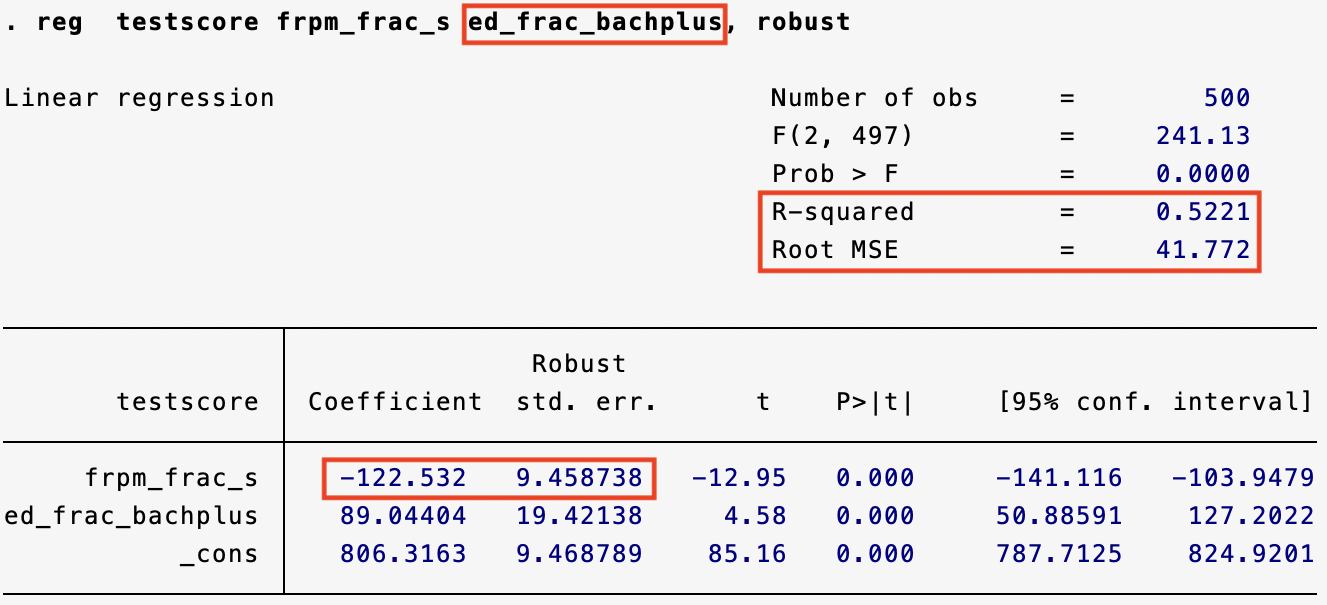
\includegraphics[scale=.6]{images/regcontr1.png}
\end{center}
\end{frame}

\begin{frame}{Tests of Joint Hypotheses }
Imagine we are interested in estimating
\begin{equation*}
    TestScore_i = \beta_0 + \beta_1 frpmfracs_i + \beta_2 edfracbachplus_i + \beta_3 strs_i + u_i
\end{equation*}

Where $strs_i$ is the student-teacher ratio in school $i$. Your theory tells you that, together with the share of subsidized meals, it captures \textit{school resources}.\\[1em]

You want to test whether \textit{school resources} matter for test scores.

\begin{eqnarray*}
    & H_0 &:= \beta_1=0 \textbf{~~AND~~} \beta_3=0\\
    VS & H_1 &:= \beta_1\neq0 \textbf{~~OR~~} \beta_3\neq0 \textbf{~~OR~~} both \\
\end{eqnarray*}


\end{frame}

\begin{frame}{Tests of Joint Hypotheses }

\begin{eqnarray*}
    & H_0 &:= \beta_1=0 \textbf{~~AND~~} \beta_3=0\\
    VS & H_1 &:= \beta_1\neq0 \textbf{~~OR~~} \beta_3\neq0 \textbf{~~OR~~} both \\
\end{eqnarray*}

\begin{itemize}
    \item A joint hypothesis specifies a value for two or more coefficients, that is, it imposes a restriction on two or more coefficients.
    \item In general, a joint hypothesis will involve $q$ restrictions. In the example, $q=2$, and the two restrictions are $\beta_1\neq0$ and $\beta_3\neq0$
    \item A ``common sense'' idea is to reject if either of the individual t-statistics exceeds 1.96 in absolute value.
    \item But this ``one at a time'' test isn’t valid: the resulting test rejects too often under the null hypothesis (more than 5\%) !
\end{itemize}

\end{frame}

\begin{frame}{Why can’t we just test the coefficients one at a time?}
\begin{itemize}
    \item Because the rejection rate under the null isn’t 5\%.
    \item We’ll calculate the probability of incorrectly rejecting the null using the ``common sense'' test based on the two individual t-statistics.
    \item To simplify suppose that $X_1$ and $X_3$ are independently distributed. Let $t_1$ and $t_3$ be 
    \begin{eqnarray*}
    & t_1 = \frac{\hat{\beta_1}}{SE(\hat{\beta_1})} \text{~~\&~~} t_3 = \frac{\hat{\beta_3}}{SE(\hat{\beta_3})}
    \end{eqnarray*}
    \item The ``one at time'' test would say we reject $H_0:= \beta_1=\beta_3=0$ if:
        \begin{eqnarray*}
    & \mid t_1 \mid > 1.96 \text{~~AND/OR~~}\mid t_3 \mid > 1.96
    \end{eqnarray*}
    \item What is the probability that this ``one at a time'' test rejects $H_0$ when $H_0$ is actually true (i.e., false positive)?    
\end{itemize}
\end{frame}

\begin{frame}{Why can’t we just test the coefficients one at a time?}
The probability of incorrectly rejecting the null hypothesis using the ``one at a time'' test (we want it to be 5\% and assume $t_1 \independent  t_3$):
\begin{eqnarray*}
    &Pr_{H_0}[\mid t_1 \mid > 1.96 \text{~~OR~~} \mid t_3 \mid > 1.96]\\
    =&1-Pr_{H_0}[\mid t_1 \mid \leq 1.96 \text{~~AND~~} \mid t_3 \mid \leq 1.96]\\
    =&1-Pr_{H_0}[\mid t_1 \mid \leq 1.96~~\times \mid t_3 \mid \leq 1.96]
\end{eqnarray*}
since $t_1$ and $t_3$ are independent by assumption.
\begin{eqnarray*}
    =&1-Pr_{H_0}[\mid t_1 \mid \leq 1.96] \times Pr_{H_0}[\mid t_3 \mid \leq 1.96]\\
    =&1-(.95)^2\\
    =&0.0975
\end{eqnarray*}
Which is way larger than the 5\%-critical value associated with the single t-test!\\

Note that we have assumed independence but in fact, its size of the test depends on the correlation between $t_1$ and $t_3$, i.e., between $\hat{\beta}_1$ and $\hat{\beta}_3$.

\end{frame}

\begin{frame}{The F-statistic}
\begin{itemize}
    \item \textbf{The solution:} use a different test statistic designed to test both ${\beta}_1$ and ${\beta}_3$ at once: the F-statistic
    \item The F-statistic tests all parts of a joint hypothesis at once.
    \item Formula for the special case of the joint hypothesis ${\beta}_1={\beta}_{1,0}$ and ${\beta}_2={\beta}_{2,0}$ in a regression with two restrictions:
    \begin{equation*}
        F=\frac{1}{2}\frac{t^2_1+t^2_2-2\hat{\rho}_{t_1, t_2}t_1t_2}{1-\hat{\rho}^2_{t_1, t_2}}
    \end{equation*}
    \item With $t_1$ and $t_2$ being independently distributed, the large-sample distribution of the F-statistic is the distribution of the average of two independently distributed squared standard normal random variables...
    \item With $q$ restrictions, the formula is more convoluted and requires softwares to be calculated
    \item We reject the null when F is large. But how large? What is the distribution of the F-stat?
\end{itemize}

\end{frame}




\begin{frame}{The $F_{q,n-k-1}$ distribution}
\begin{itemize}
    \item The F distribution is tabulated in many places
    \item As $n \rightarrow \infty$, $F_{q,n-k-1}$ distribution asymptotes to the $\chi^2_q/q$ distribution
    \item $F_{q,\infty}$ is the same as the $\chi^2_q/q$ 
     \item The chi-squared distribution with q degrees of freedom ($\chi_q^2$) is defined to be the distribution of the sum of $q$ independent squared standard normal random variables.
    \item For $q$ not too big and $n\geq 100$, the $F_{q,n-k-1}$ and the $\chi^2_q/q$ are essentially identical
    \item Many regression packages (including STATA) compute p-values of F-statistics using the F-distribution
    \item You will encounter the F distribution in published empirical work. Here, $F_{q,\infty}$:
\end{itemize}
\begin{table}[]
\begin{tabular}{|c|c|c|c|}
\hline
\rowcolor[HTML]{DAE8FC} 
{\color[HTML]{000000} \textbf{Degrees of Freedom}} & {\color[HTML]{000000} \textbf{10\%}} & {\color[HTML]{000000} \textbf{5\%}} & {\color[HTML]{000000} \textbf{1\%}} \\ \hline
1                                                  & 2.71                                 & 3.84                                & 6.63                                \\ \hline
2                                                  & 2.30                                 & 3.00                                & 4.61                                \\ \hline
3                                                  & 2.08                                 & 2.60                                & 3.78                                \\ \hline
4                                                  & 1.94                                 & 2.37                                & 3.32                                \\ \hline
5                                                  & 1.85                                 & 2.21                                & 3.02                                \\ \hline
\end{tabular}
\end{table}
\end{frame}


\begin{frame}{The $F_{q,\infty}$ distribution}
\begin{figure}
  \centering
         \vspace{-1mm}
         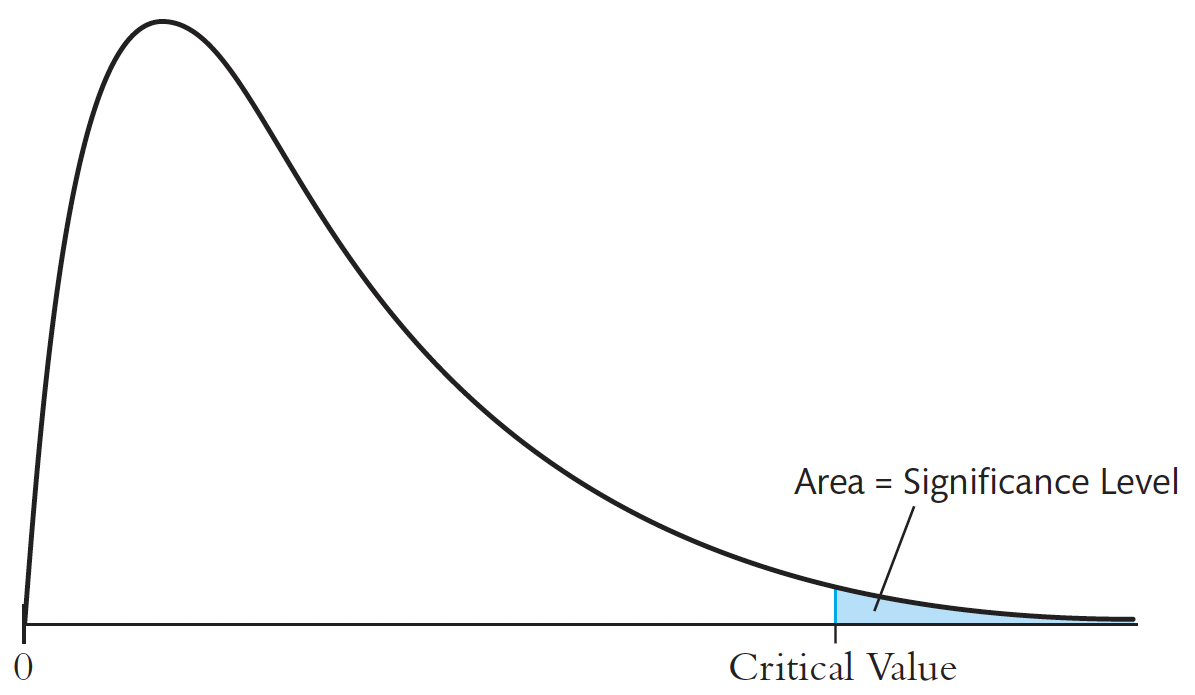
\includegraphics[scale=.6]{images/Fdist.png}
\end{figure}

\end{frame}



\begin{frame}{Interpreting Single Coefficients in Multiple Regression Analysis}
 \begin{columns}
\begin{column}{0.25\textwidth}
We can reject the null hypothesis that \textit{neither} the share of subsidized meals \textit{nor} the student-teacher ratio have an effect on test scores.
\end{column}
\begin{column}{0.8\textwidth}
\begin{figure}
  \centering
         \vspace{-1mm}
         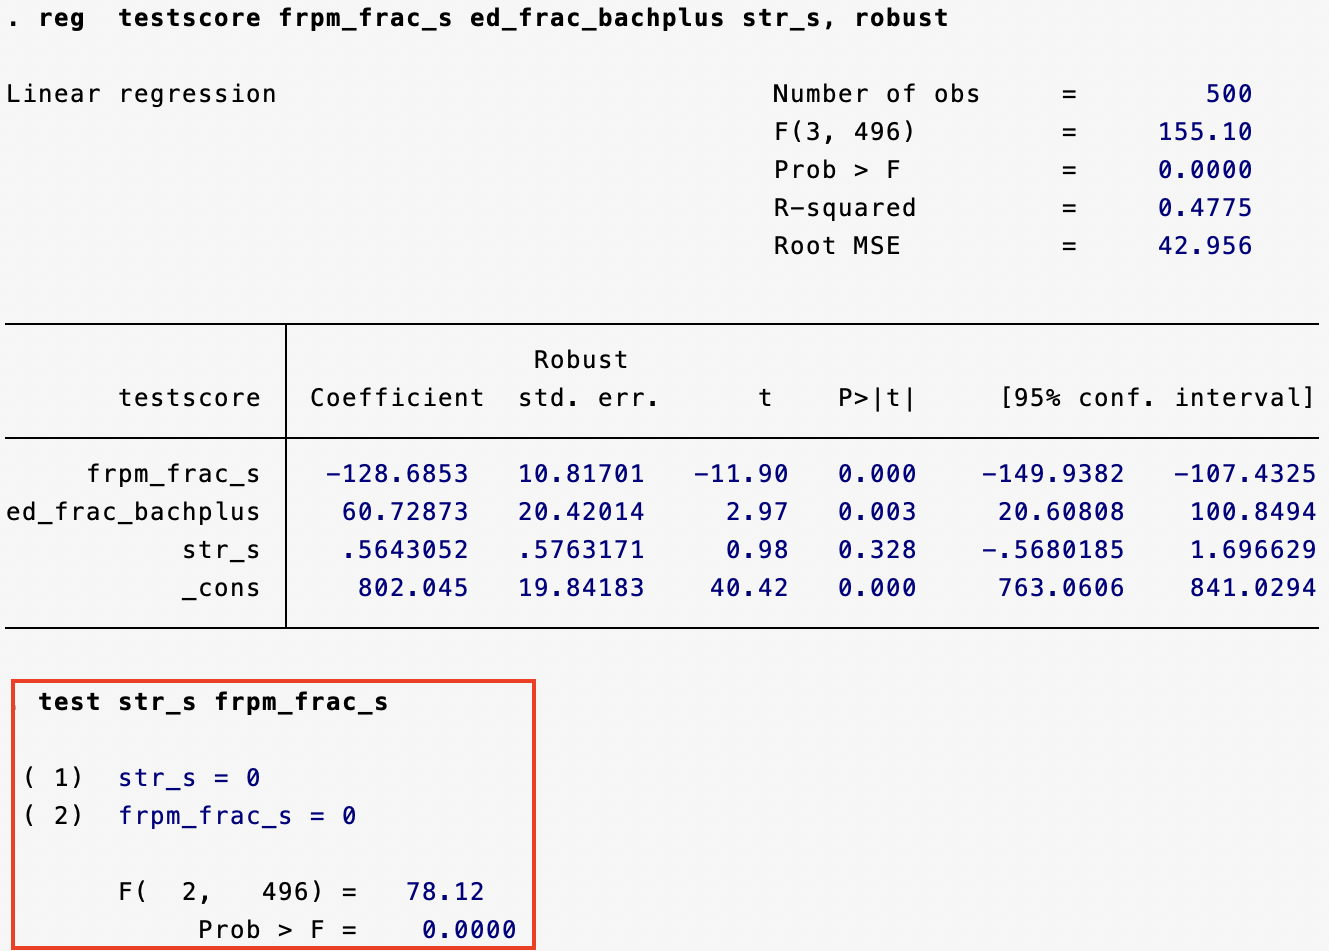
\includegraphics[scale=.45]{images/multireg1.png}
\end{figure}
\end{column}
\end{columns}
\end{frame}



\begin{frame}{The Homoskedastic-only F-statistic}
There is a simple formula for the F-statistic that holds \underline{only under homoscedasticity} (so it isn’t very useful) but which nevertheless might help you understand what the F-statistic is doing.\\[1em]

When the errors are homoscedastic, there is a simple formula for computing the ``homoscedasticity-only'' F-statistic:\\[1em]

\begin{enumerate}
    \item Run two regressions, one under the null hypothesis (the ``restricted'' regression) and one under the alternative hypothesis (the ``unrestricted'' regression).
    \item Compare the fits of the regressions –- the $R^2$'s -- if the ``unrestricted'' model fits sufficiently better, reject the null
\end{enumerate}
\end{frame}

\begin{frame}{Example: Are the coefficients on $strs$ and $frpmfracs$ zero?}


Restricted population regression (that is, under $H_0$):
\begin{equation*}
    TestScore_i = \beta_0 + \beta_2 edfracbachplus_i + u_i
\end{equation*}
\\[1em]
Unrestricted population regression (that is, under $H_1$):
\begin{equation*}
    TestScore_i = \beta_0 + \beta_1 frpmfracs_i + \beta_2 edfracbachplus_i + \beta_3 strs_i + u_i
\end{equation*}
\\[1em]
The fit will be better (higher $R^2$) in the unrestricted regression. But by how much should it be higher for $strs$ and $frpmfracs$ to be deemed statistically significantly different from zero?
\end{frame}


\begin{frame}{The Homoskedastic-only F-statistic}
\begin{equation*}
    F^{Homoskedastic-only}_q=\frac{(R^2_{unrestricted}-R^2_{restricted})/q}{(1-R^2_{unrestricted})/(n-k_{unrestricted}-1)}
\end{equation*}
where
\begin{itemize}
    \item $R^2_{unrestricted}$ is the $R^2$ for the unrestricted regression
    \item $R^2_{restricted}$ is the $R^2$ for the restricted regression
    \item $q$ is the number of restrictions under $H_0$
    \item $k_{unrestricted}$ is the number of regressors in the unrestricted regression
\end{itemize}\\[1em]
So the bigger the difference between the restricted and unrestricted $R^2$ -- i.e., the greater the improvement in fit by adding the variables in question -- the larger the homoskedasticity-only F.

\end{frame}


\begin{frame}{The Homoskedastic-only F-statistic}
\underline{\textbf{Restricted population regression (that is, under $H_0$):}}
\begin{equation*}
  \begin{alignedat}{2}
    TestScore_i = 705&.157 &{}+ 203&.582 \times edfracbachplus_i &{} + u_i\\
        (5&.106)  &   (21&.472) &
  \end{alignedat}
\end{equation*}
with $R^2_{restricted}$ = 0.2320\\[2em]
\underline{\textbf{Unrestricted population regression (that is, under $H_0$):}}
\begin{equation*}
  \begin{alignedat}{4}
    TestScore_i = 802&.045 &{} -128&.685 \times frpmfracs_i &{} +  60&.729 \times edfracbachplus_i &{}+  0&.564 \times strs_i &{}+ u_i\\
    (19&.841)  &   (10&.817) & (20&.420) & (0&.576) &
  \end{alignedat}   
\end{equation*}
with $R^2_{unrestricted}$ = 0.4775
\end{frame}

\begin{frame}{The Homoskedastic-only F-statistic}
\begin{equation*}
    F^{Homoskedastic-only}_q=\frac{(0.4775-0.2320)/2}{(1-0.4775)/(500-3-1)}=116.5244
\end{equation*}
\\[1em] whereas the heteroskedasticity-robust $F$ is
\begin{equation*}
    F_q=78.12
\end{equation*}
\begin{itemize}
    \item If the errors are a) i.i.d., b) homoskedastic, and c) normally distributed, then the homoskedasticity-only F-statistic follows an $F_{q,n-k-1}$ distribution
    \item But if the errors are heteroscedastic, the large-sample distribution of the homoscedasticity-only F-statistic is \textbf{not} $\chi^2_q/q$
\end{itemize}


\end{frame}


\begin{frame}{Why the Homoskedastic-only F-statistic?}
\begin{itemize}
    \item The theory of the homoskedasticity-only F-statistic and the $F_{q,n-k-1}$ distributions rests on implausibly strong assumptions
    \item These statistics date to the early 20th century when data sets were small and computers were people…
    \item The F-statistic and $F_{q,n-k-1}$ distribution were major breakthroughs: an easily computed formula; a single set of tables that could be published once, then applied in many settings; and a precise, mathematically elegant justification.
    \item The strong assumptions were a minor price for this breakthrough.
    \item But with modern computers and large samples we can use the heteroskedasticity-robust F-statistic and the $F_{q,\infty}$ distribution, which only require the four least squares assumptions
    \item This historical legacy persists in modern software, in which homoskedasticity-only standard errors (and F-statistics) are the default, and in which p-values are computed using the $F_{q,\infty}$ distribution
\end{itemize}
\end{frame}

\begin{frame}{Summary}
\begin{itemize}
    \item The homoskedasticity-only F-statistic and the $F_{q,n-k-1}$ distributions are justified only under very strong conditions – stronger than are realistic in practice.\\[1em]
    \item You should use the heteroskedasticity-robust F-statistic, with $F_{q,\infty}$ (i.e., $\chi^2_q/q$) critical values\\[1em]
    \item For $n\geq100$, the F-statistic distribution is essentially the $\chi^2_q/q$ distribution\\[1em]
    \item The homoskedasticity-only F-statistic is important historically (and thus in practice), and can help intuition, but isn’t valid when there is heteroskedasticity
\end{itemize}
\end{frame}


\begin{frame}{Testing Single Restrictions on Multiple Coefficients}
Consider the following specification
\begin{equation*}
    Y_i = \beta_0 + \beta_1 X_{1i}+ \beta_2 X_{2i} +u_i
\end{equation*}
and the null and alternative hypothesis,
\begin{eqnarray*}
    H_0 := \beta_1=\beta_2 \text{~~VS~~}  & H_1 &:= \beta_1\neq\beta_2
\end{eqnarray*}
This null imposes a single restriction on multiple coefficients – it is not a joint hypothesis with multiple restrictions!\\[1em]

Here are two methods for testing single restrictions on multiple coefficients:
\begin{enumerate}
    \item Rearrange the regressors so that the restriction becomes a restriction on a single coefficient in an equivalent regression; or,
    \item Perform the test directly (Some software, including STATA, lets you test restrictions using multiple coefficients directly)
\end{enumerate}
\end{frame}


\begin{frame}{Rearranging}
From the following specification
\begin{equation*}
    Y_i = \beta_0 + \beta_1 X_{1i}+ \beta_2 X_{2i} +u_i
\end{equation*}
Add and substract $ \beta_2 X_{1i}$:
\begin{eqnarray*}
    &Y_i &= \beta_0 + (\beta_1 - \beta_2)X_{1i}+ \beta_2 (X_{2i} + X_{1i}) +u_i\\
    & &= \beta_0 + \gamma_1 X_{1i}+ \beta_2 W_{i} +u_i
\end{eqnarray*}
Then test:
\begin{eqnarray*}
    H_0 := \gamma_1=0 \text{~~VS~~}  & H_1 &:= \gamma_1\neq 0
\end{eqnarray*}
The original and rearranged regressions have the same $R^2$, the same predicted values, and the same residuals, but the problem is now a simpler one.
\end{frame}


\begin{frame}{Direct Testing (here, with STATA)}
\begin{figure}
  \centering
         \vspace{-1mm}
         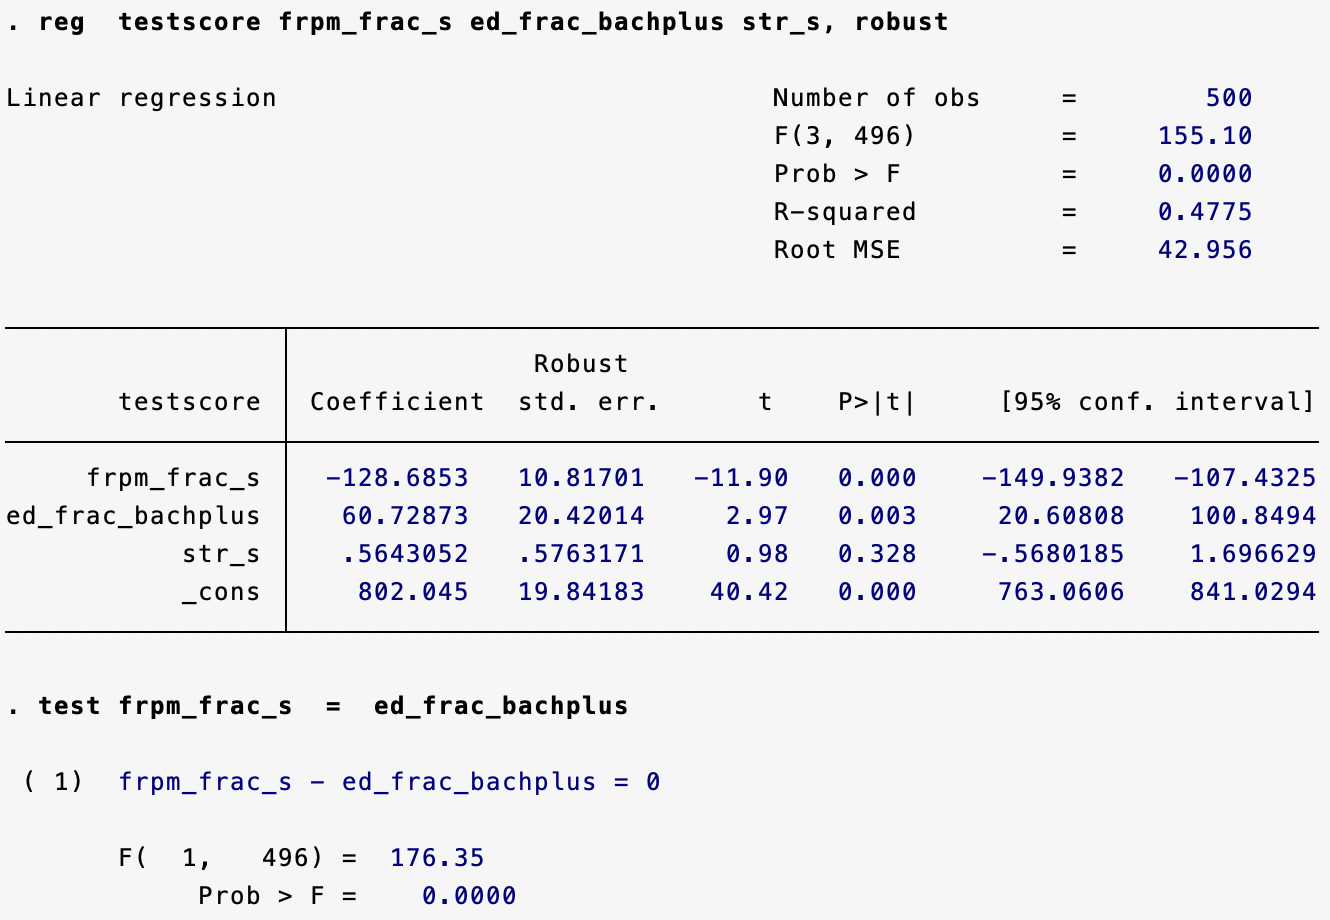
\includegraphics[scale=.45]{images/multireg3.png}
\end{figure}

\end{frame}


\begin{frame}{Confidence Sets for Multiple Coefficients}
Consider the following regression
\begin{equation*}
    Y_i = \beta_0 + \beta_1 X_{1i} + \beta_2 X_{2i} + \dots  + \beta_k X_{ki} + u_i
\end{equation*}\\[1em]

What is a joint confidence set for $\beta_1$ and $\beta_2$?\\[1em]

A 95\% joint confidence set is:
\begin{itemize}
    \item A set-valued function of the data that contains the true coefficient(s) in 95\% hypothetical repeated samples.
    \item Equivalently, the set of coefficient values that cannot be rejected at the 5\% significance level
\end{itemize}

You can find a 95\% confidence set as the set of $(\beta_1, \beta_2)$ that cannot be rejected at the 5\% level using an F-test (why not just combine the two 95\% confidence intervals?).

\end{frame}


\begin{frame}{Confidence Sets for Multiple Coefficients}
\begin{itemize}
    \item Let $F(\beta_{1,0}, \beta_{2,0})$ be the (heteroskedasticity-robust) F-statistic testing the hypothesis that $\beta_{1}=\beta_{1,0}$ and $\beta_{2}=\beta_{2,0}$\\[1em]
    \item 95\% confidence set is defined by $\{\beta_{1,0}, \beta_{2,0}: F(\beta_{1,0}, \beta_{2,0})<3.00\}$\\[1em]
    \item ... where 3.00 is the 5\% critical value of the $F_{2, \infty}$ distribution\\[1em]
    \item This set has a coverage rate of 95\% because the test on which it is based (the test it “inverts”) has a size of 5\%\\[1em]
    \item ... i.e., 5\% of the time, the test incorrectly rejects the null when the null is true, so 95\% of the time it does not; therefore the confidence set constructed as the nonrejected values contains the true value 95\% of the time (in 95\% of all samples).
\end{itemize}
\end{frame}


\begin{frame}{Confidence Sets for Multiple Coefficients}
\begin{eqnarray*}
    \biggl\{\beta_{1,0}, \beta_{2,0}: F(\beta_{1,0}, \beta_{2,0})<3.00\biggr\}\\
    \Leftrightarrow\biggl\{\beta_{1,0}, \beta_{2,0}: F=\frac{1}{2}\biggl( \frac{t_1^2+t_2^2-2\hat{\rho}_{t_1, t_2}t_1t_2}{1-\hat{\rho}^2_{t_1, t_2}}\biggr)<3.00\biggr\}\\
\end{eqnarray*}
That is,
\begin{eqnarray*}
    F=\frac{1}{2(1-\hat{\rho}^2_{t_1, t_2})} \times \biggr[\biggl( \frac{\hat{\beta}_1-\beta_{1,0}}{SE(\hat{\beta}_1)}\biggr)^2+\biggl( \frac{\hat{\beta}_2-\beta_{2,0}}{SE(\hat{\beta}_2)}\biggr)^2+ 2\hat{\rho}^2_{t_1, t_2}\biggl(\frac{\hat{\beta}_1-\beta_{1,0}}{SE(\hat{\beta}_1)}\biggr)\biggl(\frac{\hat{\beta}_2-\beta_{2,0}}{SE(\hat{\beta}_2)}\biggr)\biggr]
\end{eqnarray*}
thus the boundary of the set defined by $F<3.00$ is an ellipse.
\end{frame}


\begin{frame}{Confidence Sets for Multiple Coefficients}
\begin{figure}
  \centering
         \vspace{-1mm}
         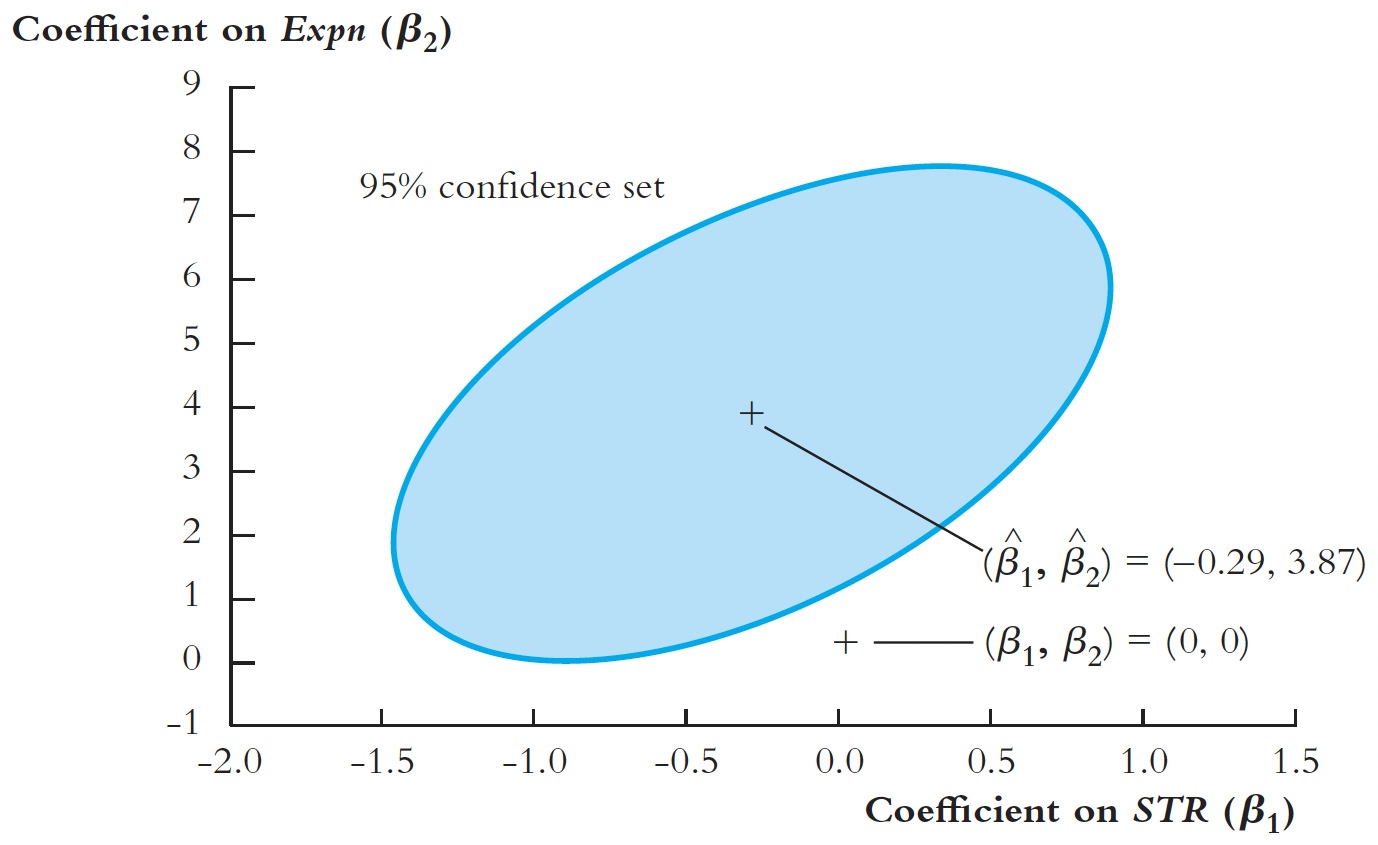
\includegraphics[scale=.5]{images/multireg_ci.png}
\end{figure}
\end{frame}


\begin{frame}{How to decide what variables to include}
\begin{enumerate}
    \item Identify the variable of interest

    \item Think of the omitted causal effects that could result in omitted variable bias

    \item Include those omitted causal effects if you can or, if you can’t, include variables correlated with them that serve as control variables.

    \begin{itemize}
        \item The control variables are effective if the conditional mean independence assumption plausibly holds, that is, if $u$ is uncorrelated with the share of subsidized meals once the control variables are included. 
        \item This results in a “base” or “benchmark” model.
    \end{itemize}

    \item Also specify a range of plausible alternative models, which include additional candidate variables.

    \item Estimate your base model and plausible alternative specifications (“sensitivity checks”).
    \begin{itemize}
        \item Does a candidate variable change the coefficient of interest $\beta_1$?
        \item Is a candidate variable statistically significant?
        \item Use judgment, not a mechanical recipe…
        \item Don’t just try to maximize the $R^2$ !
    \end{itemize}
\end{enumerate}
\end{frame}

\begin{frame}{What the $R^2$ tells you, and what it doesn't }
It is easy to fall into the trap of maximizing the $R^2$ and $\overline{R}^2$ but this loses sight of our real objective: an unbiased estimator of the class size effect.\\[1em]
\begin{itemize}
    \item A high $R^2$ (or $\overline{R}^2$) means that the regressors explain the variation in your data\\[1em]
    \item A high $R^2$ (or $\overline{R}^2$) \textbf{does not} mean that you have eliminated omitted variable bias
    \item A high $R^2$ (or $\overline{R}^2$) \textbf{does not} mean that you have an unbiased estimator of a causal effect $\beta_1$
    \item A high $R^2$ (or $\overline{R}^2$) \textbf{does not} mean that the included variables are statistically significant --- this must be determined using hypotheses tests.
\end{itemize}
\end{frame}

\begin{frame}{Summary}
\begin{itemize}
    \item Multiple regression allows you to estimate the effect on $Y$ of a change in $X_1$, holding other included variables constant.\\[1em]
    \item If you can measure a variable, you can avoid omitted variable bias from that variable by including it.\\[1em]
    \item If you can’t measure the omitted variable, you still might be able to control for its effect by including a control variable.\\[1em]
    \item There is no simple recipe for deciding which variables belong in a regression -- you must exercise judgment.\\[1em]
    \item One approach is to specify a base model -- relying on a priori reasoning -- then explore the sensitivity of the key estimate(s) in alternative specifications.
\end{itemize}

\end{frame}



\begin{frame}[allowframebreaks]{Material}
\begin{itemize}
    \item[--] \textbf{Textbooks:}
    \begin{itemize}
        \item Introduction to Econometrics, 4th Edition, Global Edition, by Stock and Watson -- Chapter 7
        \item Introductory Econometrics, 5th Edition, A Modern Approach, by Jeff. Wooldridge  -- Chapter 4-6.
    \end{itemize}
    \item[--] \textbf{Papers:}
    \begin{itemize}
        \item Krueger, A. B. (1993). How computers have changed the wage structure: evidence from microdata, 1984–1989. The Quarterly Journal of Economics, 108(1), 33-60.
        \item DiNardo, J. E., \& Pischke, J. S. (1997). The returns to computer use revisited: Have pencils changed the wage structure too?. The Quarterly Journal of Economics, 112(1), 291-303.
    \end{itemize}
\end{itemize}
\scriptsize{
\bibliographystyle{ecta}
\bibliography{base} 
}
\end{frame}




\end{document}



